%Dạng 1
\setcounter {section} {25}
\setcounter{ex}{0}
\section{Xét tính đơn điệu dựa vào bảng biến thiên của hàm số}
\subsection{Kiến thức cần nhớ}
\begin{khung} 
	\textbf{Định lý. }\\
	Cho hàm số $y=f(x)$ có đạo hàm trên $K$.
	\begin{enumerate}
		\item Nếu $f'(x)>0$ với mọi $x$ thuộc $K$ thì hàm số $f(x)$ đồng biến trên $K$.
		\item Nếu $f'(x)<0$ với mọi $x$ thuộc $K$ thì hàm số $f(x)$ nghịch biến trên $K$.
	\end{enumerate}
	\textbf{Chú ý: }
	\begin{itemize}
		\item $f(x)$  \textbf{đồng biến} trên $K$: đồ thị hàm số là \underline{đường đi lên} từ trái sang phải.
		\item $f(x)$  \textbf{nghịch biến} trên $K$: đồ thị hàm số là \underline{đường đi xuống} từ trái sang phải.
	\end{itemize}
\end{khung}
\subsection{Bài tập mẫu}
\Opensolutionfile{ans}[ans/ANS-DANG-26]
\begin{khung}
\begin{vd}[Đề tham khảo BGD 2022-2023]%[Thịnh Ngô]%[2D1Y1-2]
	Cho hàm số $y=f(x)$ có bảng biến thiên như sau\\
	\centerline{
		\begin{tikzpicture}[>=stealth]
			\def\myltespcl{3}\def\myltlgt{1.5}\def\myltdeltacl{0.5}
			\def\myltx{0.7}\def\myltya{0.7}\def\myltyb{2.1}
			\draw(\myltlgt/2,-\myltx/2) node {$x$}
			(\myltlgt/2,-\myltx-\myltya/2) node {$f'(x)$}
			(\myltlgt/2,-\myltx-\myltya-\myltyb/2) node {$f(x)$};
			\draw(0,-\myltx)--(\myltlgt+3*\myltespcl+2*\myltdeltacl,-\myltx)
			(0,-\myltx-\myltya)--(\myltlgt+3*\myltespcl+2*\myltdeltacl,-\myltx-\myltya)
			(\myltlgt,0)--(\myltlgt,-\myltx-\myltya-\myltyb);
			\draw(\myltlgt+\myltdeltacl,-\myltx/2) node {$-\infty$}
			(\myltlgt+\myltespcl+\myltdeltacl,-\myltx/2) node {$1$}
			(\myltlgt+2*\myltespcl+\myltdeltacl,-\myltx/2) node {$3$}
			(\myltlgt+3*\myltespcl+\myltdeltacl,-\myltx/2) node {$+\infty$}
			(\myltlgt+\myltdeltacl+\myltespcl/2,-\myltx-\myltya/2) node {$+$}
			(\myltlgt+\myltespcl+\myltdeltacl,-\myltx-\myltya/2) node {$0$}
			(\myltlgt+\myltdeltacl+1.5*\myltespcl,-\myltx-\myltya/2) node {$-$}
			(\myltlgt+\myltdeltacl+2*\myltespcl,-\myltx-\myltya/2) node {$0$}
			(\myltlgt+\myltdeltacl+2.5*\myltespcl,-\myltx-\myltya/2) node {$+$};
			\node (myltna) at (\myltlgt+\myltdeltacl,-\myltx-\myltya-\myltyb+\myltx/2) {$-\infty$};
			\node (myltnb) at (\myltlgt+\myltespcl+\myltdeltacl,-\myltx-\myltya-\myltx/2) {$2$};
			\node (myltnc) at (\myltlgt+2*\myltespcl+\myltdeltacl,-\myltx-\myltya-\myltyb+\myltx/2) {$0$};
			\node (myltnd) at (\myltlgt+3*\myltespcl+\myltdeltacl,-\myltx-\myltya-\myltx/2) {$+\infty$};
			\draw[->](myltna) edge (myltnb) (myltnb) edge (myltnc) (myltnc) edge (myltnd);
		\end{tikzpicture}
	}\\
	Hàm số đã cho nghịch biến trên khoảng nào dưới đây?
	\choice
	{$(0;2)$}
	{$(3;+\infty)$}
	{$(-\infty;1)$}
	{\True $(1;3)$}
	\loigiai
	{
		Dựa vào bảng biến thiên ta thấy hàm số nghịch biến trên $\left(1;3\right)$.
	}
\end{vd}

\end{khung}
\subsection{Bài tập tương tự và phát triển}
\begin{ex}%[Thịnh Ngô]%[2D1Y1-2]
	Cho hàm số $f( x )$ có bảng biến thiên như sau
	\begin{center}
		\begin{tikzpicture}
			\tkzTabInit[nocadre,lgt=1.2,espcl=2.8]
			{$x$ /0.6,$f'(x)$ /0.6,$f(x)$ /2}
			{$-\infty$,$-2$,$0$,$2$,$+\infty$}
			\tkzTabLine{,-,$0$,+,$0$,-,$0$,+,}
			\tkzTabVar{+/$+\infty$, -/$1$,+/$3$,-/$1$,+/$+\infty$}
		\end{tikzpicture}
	\end{center}
	Hàm số đã cho nghịch biến trên khoảng nào dưới đây?
	\choice 
	{\True $( 0\,;\,2 )$}
	{$( 0\,;\,+\infty )$}
	{$( -2\,;\,0 )$}
	{$( 2\,;\,+\infty )$}
	\loigiai{
		Ta có $f'( x )<0\Leftrightarrow \forall x\in (-\infty; -2)\cup ( 0; 2)$.\\
		Suy ra $f( x )$ nghịch biến trên khoảng $(-\infty; -2)$ và $( 0; 2)$.} \end{ex} 
\begin{ex}%[Thịnh Ngô]%[2D1Y1-2]
	Cho hàm số $f(x)$ có bảng biến thiên
	\begin{center}
		\begin{tikzpicture}
			\tkzTabInit[nocadre,lgt=1.2,espcl=2.8]
			{$x$ /0.6,$f'(x)$ /0.6,$f(x)$ /2}
			{$-\infty$,$1$,$3$,$+\infty$}
			\tkzTabLine{,-,$0$,+,$0$,-,}
			\tkzTabVar{+/$+\infty$, -/$-2$,+/$2$,-/$-\infty$}
		\end{tikzpicture}
	\end{center}
	Hàm số đã cho đồng biến trên khoảng
	\choice 
	{$( -\infty;1 )$}
	{$( 3;+\infty )$}
	{\True $( 1;3 )$}
	{$( -2;-2 )$}
	\loigiai{
		Quan sát bảng biến thiên đã cho nhận thấy hàm số đồng biến trên khoảng $( 1;3 )$.} \end{ex} 
\begin{ex}%[Thịnh Ngô]%[2D1Y1-2]
	Cho hàm số $y=f(x)$ có bảng biến thiên như sau
	\begin{center}
		\begin{tikzpicture}
			\tkzTabInit[nocadre,lgt=1.2,espcl=2.8]
			{$x$ /0.6,$f'(x)$ /0.6,$f(x)$ /2}
			{$-\infty$,$-1$,$0$,$1$,$+\infty$}
			\tkzTabLine{,-,$0$,+,$0$,-,$0$,+,}
			\tkzTabVar{+/$+\infty$, -/$4$,+/$-3$,-/$-4$,+/$+\infty$}
		\end{tikzpicture}
	\end{center}
	Hàm số đã cho đồng biến trên khoảng nào dưới đây?
	\choice 
	{$( -\infty;-1 )$}
	{$( 0;+\infty )$}
	{$( 0;1 )$}
	{\True $( -1;0 )$}
	\loigiai{
		Từ bảng biến thiên ta có hàm số đồng biến trên khoảng $( -1;0 )$.} \end{ex} 
\begin{ex}%[Thịnh Ngô]%[2D1Y1-2]
	Cho hàm số $y=f( x )$ có bảng xét dấu đạo hàm như hình bên dưới. Mệnh đề nào sau đây \textbf{đúng}?
	\begin{center}
		\begin{tikzpicture}
			\tkzTabInit[nocadre,lgt=1.2,espcl=2.8]
			{$x$ /0.6,$f'(x)$ /0.6}
			{$-\infty$,$-1$,$0$,$2$,$+\infty$}
			\tkzTabLine{,+,$0$,-,d,-,$0$,+,}
		\end{tikzpicture}
	\end{center}
	
	\choice 
	{Hàm số đồng biến trên khoảng $( -1;0 )$}
	{Hàm số nghịch biến trên khoảng $( 1;3 )$} 
	{Hàm số nghịch biến trên khoảng $( -1;2 )$}
	{\True Hàm số đồng biến trên khoảng $( -2;-1 )$}
	\loigiai{
		Dựa vào bảng biến thiên ta có\\
		Hàm số đồng biến trên $( -\infty;-1 )$ và $( 2;+\infty )$.\\
		Hàm số nghịch biến trên $( -1;0 )$ và $( 0;2 )$.} \end{ex} 
\begin{ex}%[Thịnh Ngô]%[2D1Y1-2]
	Cho hàm số $y=f(x)$ có bảng biến thiên như sau.
	\begin{center}
		\begin{tikzpicture}
			\tkzTabInit[nocadre,lgt=1.2,espcl=2.8]
			{$x$ /0.6,$f'(x)$ /0.6,$f(x)$ /2}
			{$-\infty$,$-3$,$2$,$+\infty$}
			\tkzTabLine{,-,$0$,+,$0$,-,}
			\tkzTabVar{+/$+\infty$, -/$2$,+/$3$,-/$-\infty$}
		\end{tikzpicture}
	\end{center}
	Hàm số đã cho đồng biến trên khoảng nào dưới đây?
	\choice 
	{$(2;3)$}
	{\True $(-3;2)$}
	{$(2;+\infty )$}
	{$(-\infty;-3)$}
	\loigiai{
		Từ bảng biến thiên suy ra hàm số đã cho đồng biến trên khoảng $(-3;2)$.}
\end{ex}
\begin{ex}%[Thịnh Ngô]%[2D1Y1-2]
	Cho hàm số $y=f( x )$ có bảng biến thiên như sau
	\begin{center}
		\begin{tikzpicture}
			\tkzTab
			[lgt=2,espcl=2] % tùy chọn
			{$x$/0.8, $f’(x)$/0.8, $f(x)$/2} % cột đầu tiên
			{$-\infty$, $-2$, $1$, $2$, $+\infty$} % hàng 1 cột 2
			{,-,0,+,d,+,0,-,} % hàng 2 cột 2
			{+/ $+\infty$, -/ $2$, +D-/ $+\infty$ / $-\infty$, +/ $3$, -/ $-\infty$} % hàng 3 cột 2
		\end{tikzpicture}
	\end{center}
	Hàm số đã cho đồng biến trên khoảng nào dưới đây?
	\choice 
	{\True $( -2\,;\,1 )$}
	{$( -2;2 )$}
	{$( -\infty;\,-2 )$}
	{$( 1\,;\,+\infty )$}
	\loigiai{
		Dựa vào bảng biến thiên ta có hàm số đồng biến trên $( -2\,;\,1 )$ và $(1;2)$.
		} 
\end{ex} 
\begin{ex}%[Thịnh Ngô]%[2D1Y1-2]
	Cho hàm số $y=f( x )$ có bảng biến thiên như sau
	\begin{center}
		\begin{tikzpicture}
			\tkzTabInit[nocadre,lgt=1.2,espcl=2.8]
			{$x$ /0.6,$f'(x)$ /0.6,$f(x)$ /2}
			{$-\infty$,$-2$,$0$,$2$,$+\infty$}
			\tkzTabLine{,+,$0$,-,$0$,+,$0$,-,}
			\tkzTabVar{-/$-\infty$, +/$3$,-/$-1$,+/$3$,-/$-\infty$}
		\end{tikzpicture}
	\end{center}
	Hàm số $y=f( x )$ nghịch biến trên khoảng nào dưới đây?
	\choice 
	{\True $( -2;\,0 )$}
	{$( -\infty;\,-2 )$} 
	{$( 0;\,2 )$}
	{$( 0;\,+\infty )$}
	\loigiai{
		Dựa vào bảng biến thiên ta thấy hàm số nghịch biến trên các khoảng $( -2;\,0 )$ và $( 2;\,+\infty )$.} \end{ex} 
\begin{ex}%[Thịnh Ngô]%[2D1Y1-2]
	Cho hàm số $f( x )$ có bảng biến thiên sau:
	\begin{center}
		\begin{tikzpicture}
			\tkzTabInit[nocadre,lgt=1.2,espcl=2.8]
			{$x$ /0.6,$f'(x)$ /0.6,$f(x)$ /2}
			{$-\infty$,$0$,$2$,$+\infty$}
			\tkzTabLine{,-,$0$,+,$0$,-,}
			\tkzTabVar{-/$-\infty$, +/$5$,-/$3$,+/$+\infty$}
		\end{tikzpicture}
	\end{center}
	Hàm số $f( x )$ đồng biến trên khoảng nào sau đây?
	\choice 
	{$( 0;+\infty )$}
	{$( 0;2 )$}
	{$( -\infty;5 )$}
	{\True $( 2;+\infty )$}
	\loigiai{
		Dựa vào bảng biến thiên suy ra hàm số đồng biến trên khoảng $( 2;+\infty )$.} \end{ex} 
\begin{ex}%[Thịnh Ngô]%[2D1Y1-2]
	Cho hàm số $y=f(x)$ có bảng biến thiên như sau
	\begin{center}
		\begin{tikzpicture}
			\tkzTabInit[nocadre,lgt=1.2,espcl=2.8]
			{$x$ /0.6,$f'(x)$ /0.6,$f(x)$ /2}
			{$-\infty$,$2$,$3$,$+\infty$}
			\tkzTabLine{,-,$0$,+,$0$,-,}
			\tkzTabVar{+/$+\infty$, -/$2$,+/$4$,-/$-\infty$}
		\end{tikzpicture}
	\end{center}
	Hàm số đã cho nghịch biến trên khoảng nào sau đây?
	\choice 
	{$(2;+\infty )$}
	{\True $(-\infty;-2)$}
	{$(2;3)$}
	{$(-2;3)$}
	\loigiai{
		Dựa vào bảng biến thiên ta có hàm số nghịch biến trên $(-\infty;-2)$.
		} 
\end{ex} 
\begin{ex}%[Thịnh Ngô]%[2D1Y1-2]
	Cho hàm số $y=f( x )$ có bảng biến thiên như hình vẽ bên dưới. Hàm số $y=f( x )$ đồng biến trên khoảng
	\begin{center}
		\begin{tikzpicture}
			\tkzTabInit[nocadre,lgt=1.2,espcl=2.8]
			{$x$ /0.6,$f'(x)$ /0.6,$f(x)$ /2}
			{$-\infty$,$0$,$1$,$+\infty$}
			\tkzTabLine{,+,$0$,-,$0$,+,}
			\tkzTabVar{-/$-\infty$, +/$0$,-/$-1$,+/$+\infty$}
		\end{tikzpicture}
	\end{center}
	\choice 
	{$( 0\,;\,+\infty )$}
	{$( 0\,;\,1 )$}
	{\True $( -3\,;\,-2 )$}
	{$( -1\,;\,+\infty )$}
	\loigiai{
		Từ bảng biến thiên ta thấy hàm số $y=f( x )$ đồng biến trên các khoảng $( -\infty \,;\,0 )$ và $( 1;+\infty \, )$.\\
		Ta có $( -3\,;\,-2 )\subset ( -\infty \,;\,0 )$ nên hàm số đồng biến trên khoảng $( -3\,;\,-2 )$.
} \end{ex}
\begin{ex}%[Thịnh Ngô]%[2D1Y1-2] 
	Cho hàm số $y=f( x )$ có bảng biến thiên như sau
	\begin{center}
		\begin{tikzpicture}
			\tkzTabInit[nocadre,lgt=1.2,espcl=2.5,deltacl=0.6]
			{$x$/0.6,$y'$/0.6,$y$/2}
			{$-\infty$,$-3$,$-2$,$-1$,$+\infty$}
			\tkzTabLine{,+,0,-,d,-,0,+,}
			\tkzTabVar{-/$-\infty$,+/$0$,-D+/$-\infty$/$+\infty$,-/$0$,+/$+\infty$}
		\end{tikzpicture}
	\end{center}
	Hàm số đã cho nghịch biến trên khoảng nào dưới đây?
	\choice 
	{ $( -\infty ;-3 )$}
	{ \True $( -3;-2 )$}
	{ $( -3;-1 )$}
	{ $( -1;+\infty )$}
	\loigiai{
		Từ bảng biến thiên ta thấy hàm số nghịch biến trên khoảng $( -3;-2 )$.} \end{ex} 
\begin{ex}%[Thịnh Ngô]%[2D1Y1-2] 
	Cho hàm số $f(x)$có bảng biến thiên như sau
	\begin{center}
		\begin{tikzpicture}
			\tkzTabInit[nocadre,lgt=1.2,espcl=2.5,deltacl=0.6]
			{$x$/0.6,$f'(x)$/0.6,$f(x)$/2}
			{$-\infty$,$-1$,$0$,$1$,$+\infty$}
			\tkzTabLine{,-,0,+,0,-,0,+,}
			\tkzTabVar{+/$+\infty$,-/$2$,+/$3$,-/$2$,+/$+\infty$}
		\end{tikzpicture}
	\end{center} 
	Hàm số đã cho đồng biến trên khoảng nào dưới đây?
	\choice 
	{ $( -\infty;1 )$}
	{ $( 0;1 )$}
	{ $( -2;3 )$}
	{ \True $( 1;+\infty )$}
	\loigiai{
		Dựa vào bảng biến thiên của hàm số $f(x)$ ta có hàm số $f(x)$ đồng biến trên $( 1;+\infty )$.} \end{ex} 
\begin{ex}%[Thịnh Ngô]%[2D1Y1-2] 
	Cho hàm số $y=f(x)$có bảng biến thiên như sau
	\begin{center}
		\begin{tikzpicture}
			\tkzTabInit[nocadre,lgt=1.2,espcl=2.5,deltacl=0.6]
			{$x$/0.6,$y'$/0.6,$y$/2}
			{$-\infty$,$-1$,$1$,$+\infty$}
			\tkzTabLine{,-,0,+,0,-,}
			\tkzTabVar{+/$+\infty$,-/$-2$,+/$2$,-/$-\infty$}
		\end{tikzpicture}
	\end{center}
	Mệnh đề nào dưới đây \textbf{sai}?
	\choice 
	{ Hàm số $y=f(x)$ đồng biến trên khoảng $( -1;1 )$} 
	{ Hàm số $y=f(x)$ nghịch biến trên khoảng $( 1;+\infty )$} 
	{ Hàm số $y=f(x)$ nghịch biến trên khoảng $( -\infty;-1 )$} 
	{ \True Hàm số $y=f(x)$ đồng biến trên khoảng $( -2;2 )$
	}
	\loigiai{
		Từ BBT suy ra hàm số $y=f(x)$ vừa nghịch biến vừa đồng biến trên khoảng $( -2;2 )$.
		\begin{center}
			\begin{tikzpicture} 
				\tikzset{double style/.append style = {double distance=2pt}}
				\tkzTabInit[nocadre,espcl=4]
				{$x$ / 1 , $y'$ / 1, $y$ / 2} 
				{$-\infty$, $-1$ , $1$, $+\infty$} 
				\tkzTabLine{,-,0,+,0,-,} 
				\tkzTabVar{+/$+\infty $, - / $-2 $, + / $2 $, -/$ -\infty$ } 
				\tkzTabVal[draw]{4}{3}{.5}{$2$}{} 
				\tkzTabVal[draw]{1}{2}{.5}{$-2$}{} 
			\end{tikzpicture}
		\end{center}
} \end{ex} 
\begin{ex}%[Thịnh Ngô]%[2D1Y1-2] 
	Cho hàm số $y=f( x )$ có bảng biến thiên như hình vẽ
	\begin{center}
		\begin{tikzpicture}
			\tkzTabInit[nocadre,lgt=1.2,espcl=3.5,deltacl=0.6]
			{$x$/0.6,$f'(x)$/0.6,$f(x)$/2}{$-\infty$,$2$,$+\infty$}
			\tkzTabLine{,+,d,+,}
			\tkzTabVar{-/$1$,+D-/$+\infty$/$-\infty$,+/$3$}
		\end{tikzpicture}
	\end{center}
	Hàm số đã cho đồng biến trên khoảng nào dưới đây?
	\choice 
	{ \True $( 2;+\infty )$}
	{ $( 1;+\infty )$}
	{ $( -\infty;3 )$}
	{ $( -\infty;+\infty )$}
	\loigiai{
		Quan sát bảng biến thiên, ta thấy hàm số đồng biến trên mỗi khoảng $( -\infty;2 )$ và $( 2;+\infty )$, vậy hàm số đồng biến trên khoảng $( 2;+\infty )$.} \end{ex} 
\begin{ex}%[Thịnh Ngô]%[2D1Y1-2] 
	Cho hàm số $y=f( x )$ có bảng biến thiên như hình bên dưới
	\begin{center}
		\begin{tikzpicture}
			\tkzTabInit[nocadre,lgt=1.2,espcl=2.5,deltacl=0.6]
			{$x$/0.6,$y'$/0.6,$y$/2}{$-\infty$,$-2$,$0$,$2$,$+\infty$}
			\tkzTabLine{,-,0,+,d,+,0,-,}
			\tkzTabVar{+/$+\infty$,-/$3$,+D-/$+\infty$/$-\infty$,+/$1$,-/$-\infty$}
		\end{tikzpicture}
	\end{center}
	Hàm số $y=f( x )$ đồng biến trên khoảng nào dưới đây?
	\choice 
	{ $( -\infty;1 )$}
	{ $( -2;2 )$}
	{ \True $( 0;2 )$}
	{ $( 3;+\infty )$}
	\loigiai{Quan sát bảng biến thiên, ta thấy hàm số đồng biến trên mỗi khoảng  $( -2; 0)$ và  $(0; 2 )$, vậy hàm số đồng biến trên khoảng $( 0;2 )$.
} \end{ex} 
\begin{ex}%[Thịnh Ngô]%[2D1Y1-2] 
	Hàm số $y=f( x )$ có bảng biến thiên như sau
	\begin{center}
		\begin{tikzpicture}
			\tkzTabInit[nocadre,lgt=1.2,espcl=2.5,deltacl=0.6]
			{$x$/0.6,$f'(x)$/0.6,$f(x)$/2}{$-\infty$,$-2$,$1$,$+\infty$}
			\tkzTabLine{,+,0,-,0,+,}
			\tkzTabVar{-/$-\infty$,+/$1$,-/$-3$,+/$+\infty$}
		\end{tikzpicture}
	\end{center}
	Hàm số đã cho đồng biến trên khoảng
	\choice 
	{ \True $( 2;3 )$}
	{ $( -2;3 )$}
	{ $( -3;+\infty )$}
	{ $( -\infty;1 )$}
	\loigiai{
		Theo BBT hàm số đồng biến trên khoảng $( 2;3 )$.} \end{ex} 
\begin{ex}%[Thịnh Ngô]%[2D1Y1-2] 
	Cho hàm số $y=f( x )$ có bảng biến thiên như sau
	\begin{center}
		\begin{tikzpicture}
			\tkzTabInit[nocadre,lgt=1.2,espcl=2.5,deltacl=0.6]
			{$x$/0.6,$y'$/0.6,$y$/2}{$-\infty$,$-2$,$0$,$2$,$+\infty$}
			\tkzTabLine{,-,0,+,0,-,0,+,}
			\tkzTabVar{+/$+\infty$,-/$-2$,+/$1$,-/$-2$,+/$+\infty$}
		\end{tikzpicture}
	\end{center} 
	Hàm số đã cho nghịch biến trên khoảng nào dưới đây?
	\choice 
	{ $( -\infty;0 )$}
	{ \True $( 0;2 )$}
	{ $( 2;+\infty )$}
	{ $( -2;2 )$}
	\loigiai{
		Theo BBT hàm số đồng biến trên khoảng $( 0;2 )$.} \end{ex} 
\begin{ex}%[Thịnh Ngô]%[2D1Y1-2] 
	Cho hàm số $f( x )$có bảng biến thiên như sau
	\begin{center}
		\begin{tikzpicture}
			\tkzTabInit[nocadre,lgt=1.2,espcl=2.5,deltacl=0.6]
			{$x$/0.6,$y'$/0.6,$y$/2}{$-\infty$,$-1$,$0$,$1$,$+\infty$}
			\tkzTabLine{,-,0,+,0,-,0,+,}
			\tkzTabVar{+/$+\infty$,-/$-2$,+/$0$,-/$-2$,+/$+\infty$}
		\end{tikzpicture}
	\end{center}  
	Hàm số đã cho đồng biến trên khoảng nào dưới đây?
	\choice 
	{ $( 0;1 )$}
	{ \True $( -1;0 )$}
	{ $( -2;0 )$}
	{ $( 0;+\infty )$}
	\loigiai{
		Theo bảng biến thiên hàm số $f( x )$ đồng biến trên các khoảng $( -1;0 )$ và $( 1;+\infty )$.\\
		Do đó hàm số đồng biến trên $( -1;0 )$.} \end{ex} 
\begin{ex}%[Thịnh Ngô]%[2D1Y1-2] 
	Cho hàm số $y=f( x )$ xác định và liên tục trên khoảng $( -\infty ;+\infty )$, có bảng biến thiên như hình sau
	\begin{center}
		\begin{tikzpicture}
			\tkzTabInit[nocadre,lgt=1.2,espcl=2.5,deltacl=0.6]
			{$x$/0.6,$y'$/0.6,$y$/2}{$-\infty$,$-1$,$1$,$+\infty$}
			\tkzTabLine{,+,0,-,0,+,}
			\tkzTabVar{-/$-\infty$,+/$2$,-/$-1$,+/$+\infty$}
		\end{tikzpicture}
		
	\end{center}
	
	Mệnh đề nào sau đây đúng?
	\choice 
	{ Hàm số nghịch biến trên khoảng $( 1;+\infty )$}
	{ Hàm số đồng biến trên khoảng $( -1;+\infty )$} 
	{ \True Hàm số đồng biến trên khoảng $( -\infty ;-1 )$}
	{ Hàm số nghịch biến trên khoảng $( -\infty ;1 )$}
	\loigiai{
		Dựa vào bảng biến thiên ta thấy hàm số đồng biến trên khoảng $( -\infty ;-1 )$.} \end{ex} 
\begin{ex}%[Thịnh Ngô]%[2D1Y1-2] 
	Cho hàm số $y=f( x )$ có bảng biến thiên như hình vẽ bên dưới
	\begin{center}
		\begin{tikzpicture}
			\tkzTabInit[nocadre,lgt=1.2,espcl=3.5,deltacl=0.6]
			{$x$/0.6,$y'$/0.6,$y$/2}{$-\infty$,$-1$,$+\infty$}
			\tkzTabLine{,+,d,+,}
			\tkzTabVar{-/$2$,+D-/$+\infty$/$-\infty$,+/$2$}
		\end{tikzpicture}
		
	\end{center}
	Mệnh đề nào sau đây đúng?
	\choice 
	{ \True Hàm số đồng biến trên khoảng $( -\infty ;-1 )$}
	{ Hàm số đồng biến trên $\mathbb{R}\backslash \left\{ -1 \right\}$} 
	{ Hàm số đồng biến trên $\mathbb{R}$}
	{ Hàm số đồng biến trên khoảng $( -\infty ;2 )$}
	\loigiai{
		Nhìn vào bảng biến thiên ta thấy ${y}'>0,$ $\forall x\ne -1$. \\Từ đó suy ra hàm số luôn đồng biến trên các khoảng $( -\infty ;-1 )$ và $( -1;+\infty )$.} \end{ex}
\Closesolutionfile{ans}
%======================
\subsection{Bảng đáp án}
\inputansbox{10}{ans/ANS-DANG-26}


